% CNN Definition
\begin{frame}[allowframebreaks]{CNN - Definition}
\begin{itemize}
    \item Convolutional Neural Networks (CNNs) are a class of deep learning models specifically designed for processing structured grid data, such as images.
    \item They are particularly effective for tasks like image classification, object detection, and segmentation.
    \item CNNs leverage the spatial structure of images by using convolutional layers to automatically learn hierarchical features.
    \item The architecture typically consists of convolutional layers, activation functions, pooling layers, and fully connected layers.
    \item CNNs are known for their ability to capture local patterns and translate them into higher-level representations.
\end{itemize}
\end{frame}  

\begin{frame}{CNN Architecture}
    \textbf{What is a CNN?}
    
     A CNN is a deep network of neurons with learnable filters that perform convolution operations on inputs, usually images, to extract hierarchical features.
    
    \begin{figure}
    % Download at compile time
    % \fetchimage{images/cnn-arch.png}{https://vitalflux.com/wp-content/uploads/2021/11/VGG16-CNN-Architecture.png}
    \centering
    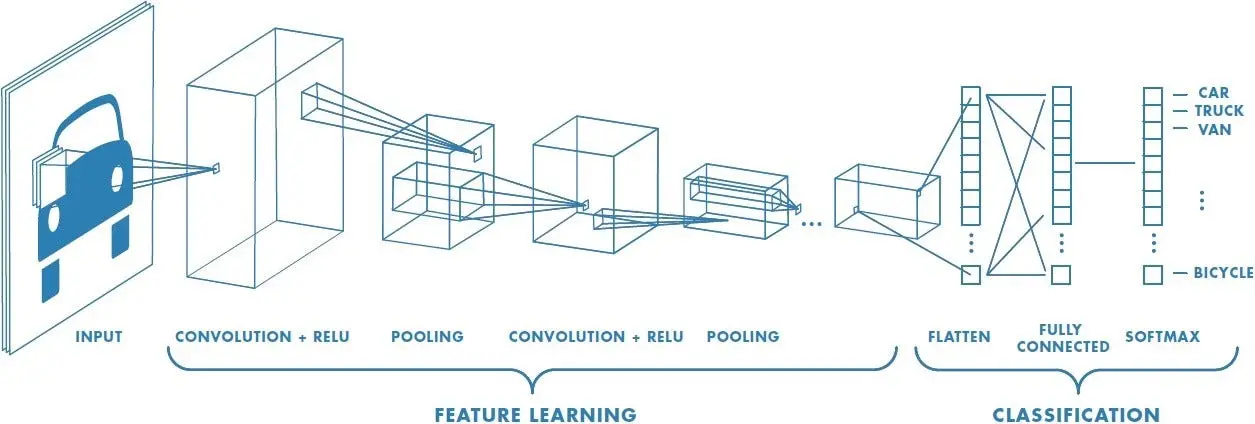
\includegraphics[width=0.8\textwidth,height=0.4\textheight,keepaspectratio]{images/cnn/cnn-architecture.png}
    \end{figure}
    \newline
    \left

    \textbf{Why use CNNs?}
    
    Parameter sharing and sparse connectivity reduce number of parameters and improve spatial feature extraction.
\end{frame}

\begin{frame}{CNN Architecture}
    \textbf{What makes a Convolutional Neural Network?}
    
    Characterised by “Convolutional Layer” – they are able to detect “abstract features” and “almost ideas within the image”

    \newline

    \begin{figure}
    \centering
    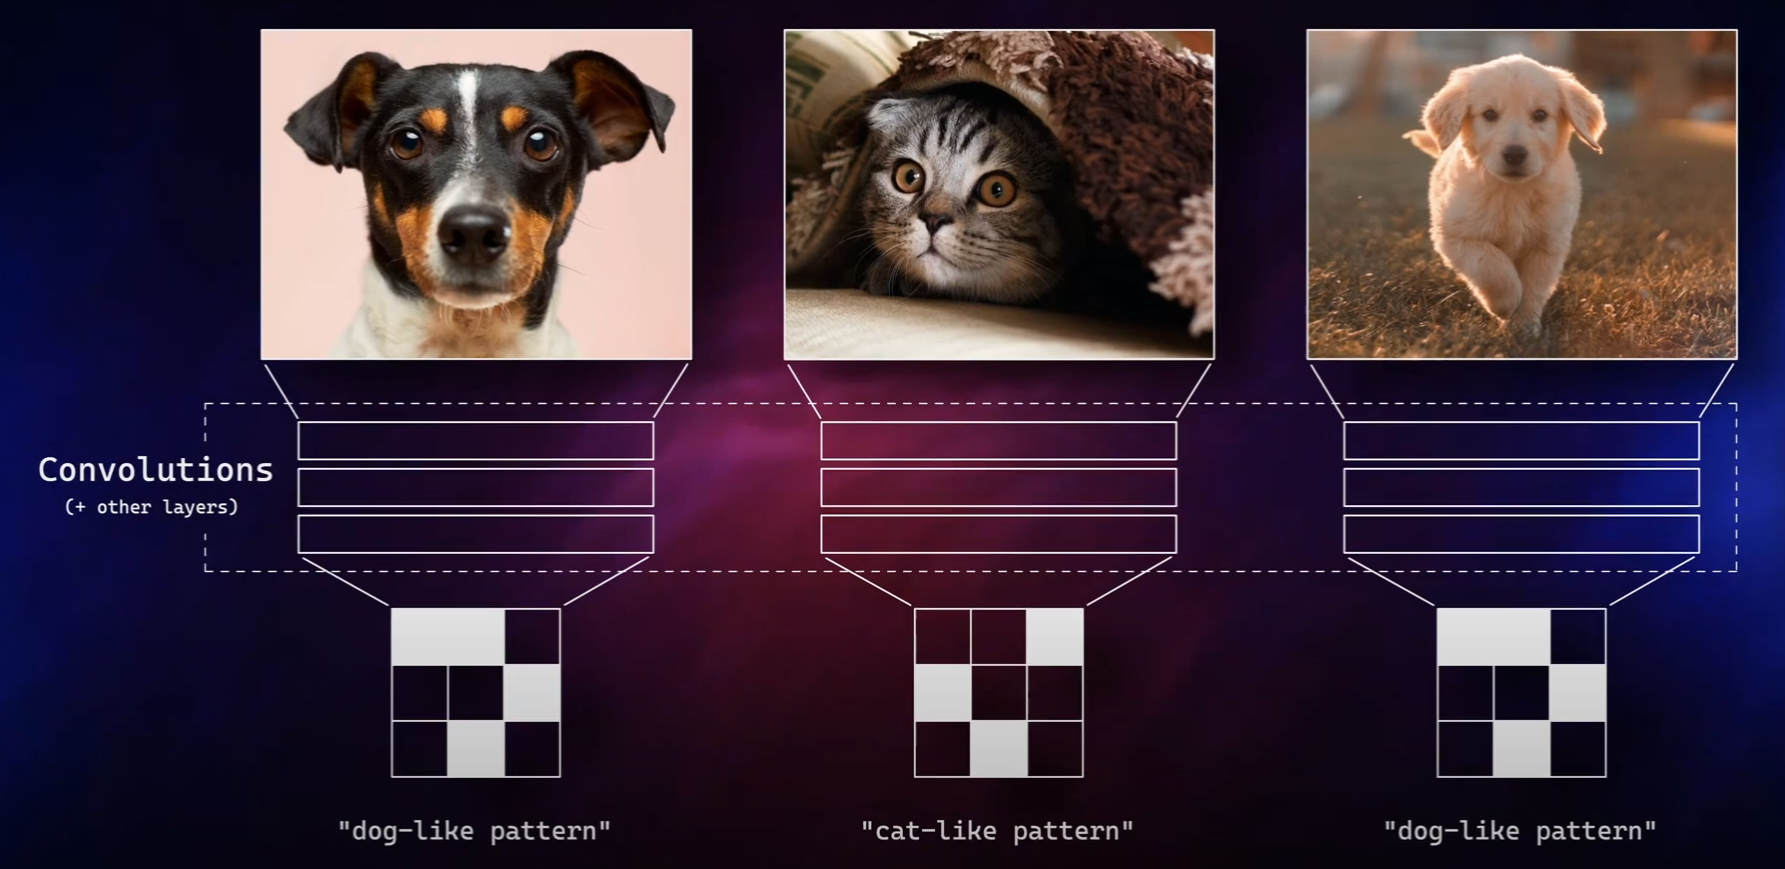
\includegraphics[width=0.8\textwidth,height=0.75\textheight,keepaspectratio]{images/cnn/what-makes-cnn.png}
    \end{figure}
\end{frame}

\begin{frame}{Components of a CNN}
    \begin{figure}
    \centering
    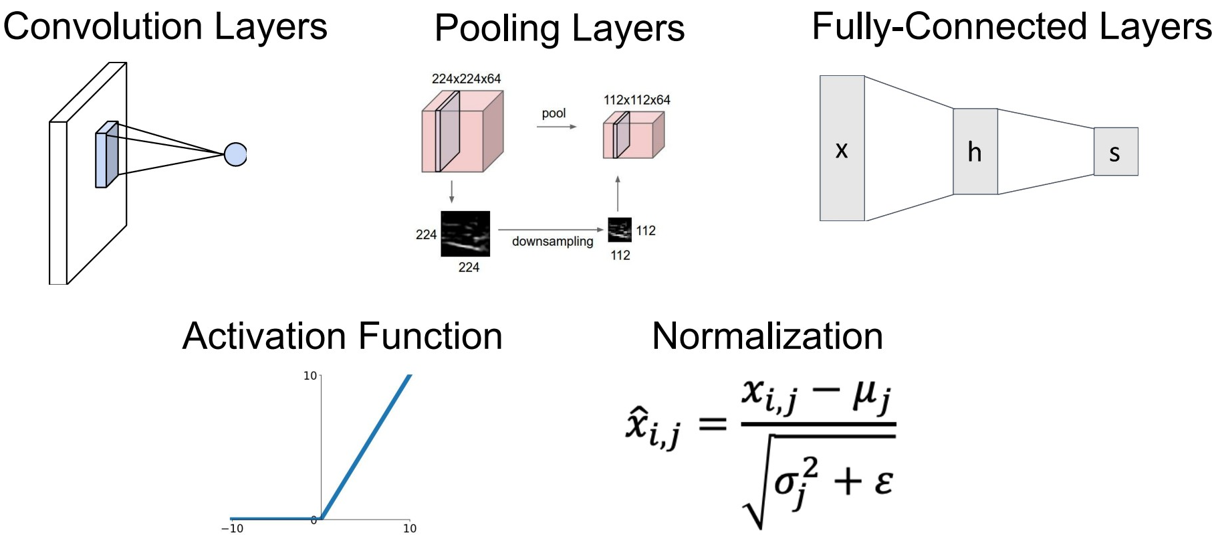
\includegraphics[width=0.95\textwidth,height=0.95\textheight,keepaspectratio]{images/cnn/cnn-components.png}
    \end{figure}
\end{frame}